\documentclass[12pt,a4paper,twocolumn]{article}
\usepackage[utf8]{inputenc}
\usepackage{amsmath}
\usepackage{amsfonts}
\usepackage{amssymb}
\usepackage{graphicx}
\usepackage{authblk}
\usepackage[font=small,labelfont=bf]{caption}

\title{``How Prolific Are You?": A Scientometric Analysis of Researchers}

\author[1]{Rahul Yedida}
\author[1]{Snehanshu Saha}
\affil[1]{Department of Computer Science \& Engineering, PESIT South Campus}

\date{}
\begin{document}
\maketitle

\abstract{
	Scholars in academia regularly write papers showing the results of their work. To gauge how relevant their work is, several measures are used, including citation count and the h-index. This paper describes the methods used to identify ``prolific" authors, whose metrics are significantly higher than their peers, and provides a general discussion of the relationships between different metrics. We also discuss how this analysis is performed even with the high dimensionality of the dataset.
}

\section{Introduction}
\underline{Give an introduction here}. 

The rest of the paper is structured as follows. Section 2 describes the data and shows correlations between the attributes. Section 3 discusses the methods we used to analyse this data.

\section{Data}
The data contains 618 records of scholars with 25 attributes. There are no missing values, and eight of the attributes are integers. For ease of analysis, we have labeled the attributes as \textit{v1} through \textit{v25}. \underline{[maybe show what these are in a table]}.

\subsection{Preliminary Analysis}
For a preliminary analysis of the relationships between the attributes, we sought to discover monotonic relationships. This was done by computing pairwise Spearman's rank correlation coefficient. This revealed that there were only positive monotonic relationships. 42.08\% of these coefficients were above 0.8, and 52\% were above 0.7.

A logical next step, then, was to investigate the percentage of linear relationships among these. This was done by computing pairwise Pearson correlation coefficients. To visually understand pairs that had high linear correlations, we displayed this information in a matrix, maintaining only the upper half, and avoiding diagonal entries. This avoids counting self-correlations and counting the same pair twice. Further, when finding multiple linear regression equations, this finds only unique relations between the variables. Figure 1 shows this result. Asterisks indicate a Pearson R value of 0.8 or higher. The numbers at the right indicate how many other variables each variable is highly correlated with. \\

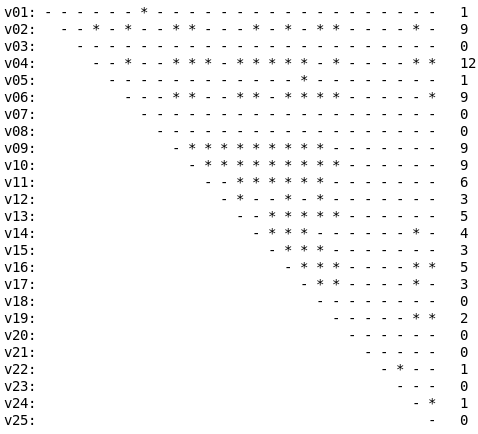
\includegraphics[scale=0.4]{fig1.png}
\begingroup
\captionof{figure}{Matrix showing pairs with Pearson R values 0.8 or higher}
\endgroup
\hfill\break
These correlations provide a starting point to find relationships between the attributes.

\section{Methods}
This section discusses in detail the methods used to analyse the data.

\subsection{Regression Analysis}
Our first analysis investigated the precise relationships between the attributes. We looked at linear relationships. Because v4 had the most number of correlations, we started with it.

Multiple regression analysis was performed as follows. For each attribute that the variable being analysed has a high correlation with, we ran an Ordinary Least Squares (OLS) regression model in two cases--with a constant term and without (that is, in a forward step-wise fashion). 

In each case, for each variable, we check the p-value to ensure that all variables are statistically significant. Finally, we choose the model with the highest adjusted $R^2$ value, which avoids the pitfalls of ``kitchen sink regression". We also make sure that there are no significant autocorrelations, using the Durbin-Watson test. \cite{field2009discovering} suggests that a conservative range for the acceptable values for this test is between 1 and 3. In some cases, we chose to pick a model that has a slightly lesser adjusted $R^2$ value in favor of using lesser variables. This results in a model that still has a high predictive power, yet is simpler. In addition, we also check the residuals vs. fits plots and check that they are not very correlated.

The full regression results can be found in the Supplementary Materials section at the end of this paper. Here, we present a summary of the results of the regression analysis that was performed.

\subsubsection{Analysis on the full data}
We first looked at v4, and did a step-wise regression analysis. \textit{v6, v9, v11, v13, v14, v17, v19, v24,} and \textit{v25} were statistically significant, and the adjusted $R^2$ was 0.972. For this model, the Durbin-Watson statistic was 2.06, which suggests very minor negative autocorrelations. The correlations between the residuals and the fitted values was -0.0047. Figure 2 shows the residuals vs. fits plot for \textit{v4}.\\

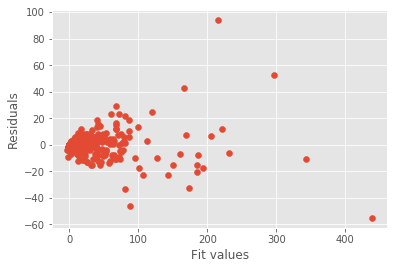
\includegraphics[scale=0.5]{fig2.png}
\begingroup
\captionof{figure}{Residuals vs. fits plot for v4}
\endgroup
\hfill\break

Our next variable of interest was \textit{v2}, having high Pearson R correlations with nine other variables. Only \textit{v9} was not statistically significant. However, we also chose to discard \textit{v24} because it added no predictive power to the model, and the adjusted $R^2$ for this model was 0.993, and the Durbin-Watson statistic was 1.853, suggesting only minor positive autocorrelations. All the p-values were less than $10^{-3}$. The correlation between the residuals and the fits was 0.023. Figure 3 shows the residuals vs. fits plot for \textit{v2}.

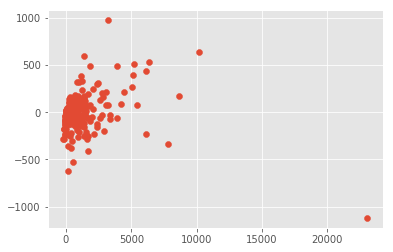
\includegraphics[scale=0.5]{fig3.png}
\begingroup
\captionof{figure}{Residuals vs. fits plot for v2}
\endgroup
\hfill\break

We then looked at \textit{v6}, also having high correlations with nine other variables. \textit{v9} and \textit{v14} were not statistically significant. We also discarded \textit{v25} to obtain a simpler model with an adjusted $R^2$ value 0.001 less. This model had an adjusted $R^2$ of 0.913, and a Durbin-Watson statistic of 1.64. All p-values were below $10^{-3}$.

Next, we looked at \textit{v9}. Only \textit{v13} was not statistically significant, but we also discarded \textit{v10} and \textit{v11}, which resulted in a model whose adjusted $R^2$ was 0.986 (a reduction of 0.002 from when the two variables were included). This model had a Durbin-Watson statistic of 1.99.

Finally, for \textit{v10}, all the predictor variables were statistically significant, and we discarded \textit{v19}, which resulted in a model with the same adjusted $R^2$. All the p-values were below $10^{-3}$, except \textit{v13}, whose p-value was 0.043 (95\% C.I [0.07, 0.425]). The Durbin-Watson statistic was 1.861.

It should be noted that in all of the regression results of the above variables, the constant was not statistically significant, and the results reported are those for the models that did not include the constant.

\subsubsection{Analysis on subset of the data}
Our next step of analysis was to pick a subset of the variables, and redo the same analysis discussed above on this subset. Once again, it turns out that for all the regression equations obtained, the constant was not statistically significant.

The variables we chose were \textit{v9} through \textit{v21} and \textit{v24}. \underline{maybe explain why these}. Again, we created a matrix of Pearson R correlations, and picked out those that were higher than 0.8. Figure 4 shows this result. \\

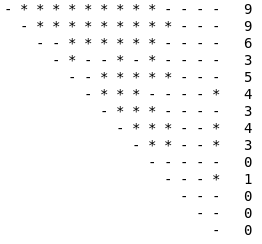
\includegraphics[scale=0.6]{fig4.png}
\begingroup
\captionof{figure}{Pearson R correlation matrix for subset of the data}
\endgroup
\hfill\break

Using this, we redid the same analysis as in the previous subsection. Again, we only discuss the results here, but the full list of experiments is in the Supplementary Materials section.

We first looked at v9. \textit{v13} was not significant when all the variables it was correlated to were considered. However, when \textit{v10} was not considered, it was statistically significant. We chose to sacrifice 0.2\% adjusted $R^2$ in favor of a model that had two fewer predictor variables. The Durbin-Watson value was 1.99.

While predicting \textit{v10}, dropping \textit{v19} resulted in no loss of adjusted $R^2$. We further dropped \textit{v18}, and dropped \textit{v12} because it was not significant. While dropping \textit{v18} caused a 0.3\% drop in adjusted $R^2$, we were able to use two less variables. The Durbin-Watson statistic was 1.991.

We only looked at two other variables, because the adjusted $R^2$ for the others was below 0.95. For \textit{v11}, dropping \textit{v17} and \textit{v18} resulted in a 0.2\% drop in adjusted $R^2$, and we were able to use only four variables to get an adjusted $R^2$ of 0.971 and a Durbin-Watson of 2.081. Finally, for \textit{v13}, all variables were statistically significant, and we discarded \textit{v19} with no loss of adjusted $R^2$.

Perhaps more interesting than the above results was when we plotted the maximum adjusted $R^2$ (without discarding any variables) against the number of predictor variables used (on this subset of the data). Figure 5 shows this result, where a logarithm function fits quite well to the data. The equation obtained was
\begin{equation}
	\text{Adj. } R^2 = 0.125465 \log n + 0.746654
\end{equation}

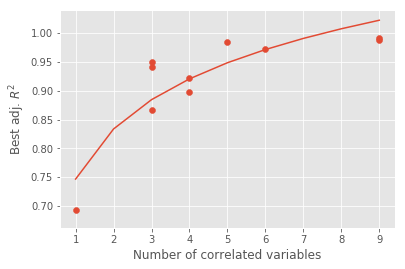
\includegraphics[scale=0.5]{fig5.png}
\begingroup
\captionof{figure}{Adjusted $R^2$ vs. number of predictor variables}
\endgroup
\hfill\break

The sum of the squared residuals for this fit was 0.01456.

\bibliographystyle{ieeetr}
\bibliography{citations}
\end{document}